\section{\emph{App Server}}
\label{sec:appserver}
Dieser Abschnitt behandelt das Openshift Projekt \emph{Appserver}, das die gebauten Services beinhaltet. Die Jenkins Pipeline löst nach dem Bauen und Veröffentlichen des Artefakts wird im Openshift Projekt \emph{Appserver} eine \emph{Build}-Konfiguration ausgelöst, die das Docker Image mit dem freigegebenen Artefakts baut. Wenn der \emph{Build} fertiggestellt ist, dann wird ein \emph{Trigger} bei der \emph{Deploy}-Konfiguration ausgelöst, der aus dem gebauten Docker Image den neuen Service einspielt.  

\begin{figure}[H]
	\centering
	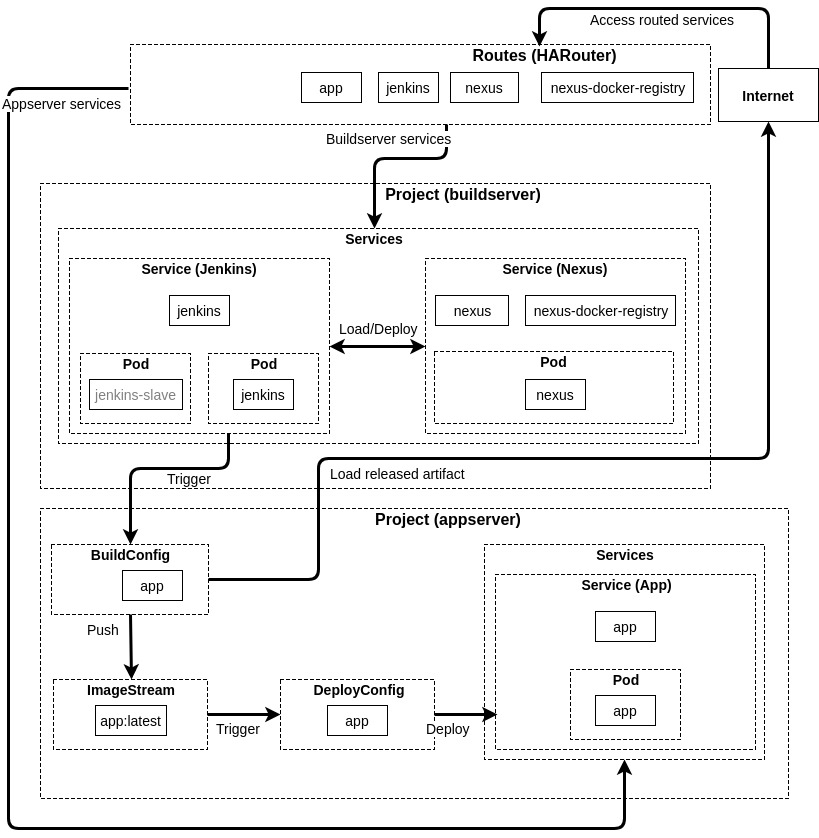
\includegraphics[scale=0.55]{logos/architecture-diagram-appserver.jpg}
	\caption{\emph{Build Server} Architektur}
	\label{fig:appserver-deploy}
\end{figure}
\ \\
Die Abbildung \ref{fig:appserver-deploy} illustriert das Zusammenspiel der beteiligten Openshift Artefakte und Services aus mehreren Projekten. In der It\&Tel \emph{Cloud}, ist es nicht möglich gewesen einen \emph{Service Account} die \emph{EDIT} Rolle zu zuweisen und einen \emph{API-Token} zu bekommen. Dadurch ist es Jenkins nicht möglich auf Artefakte des Projektes \emph{Appserver} zu zugreifen und dort \emph{Builds} zu starten. \\

Daher wird der Service im \emph{Buildserver} Projekt eingespielt, denn in diesem Projekt hat Jenkins die \emph{EDIT} Rolle. Der Prozess des Service \emph{Releases} ändert sich dadurch aber nicht. 